\section{Discussão}\label{sec:discussao}

Esta seção discute \textit{por que} o método é capaz de fazer o que os resultados mostram, e por que deixa de ser capaz em outros casos. As propriedades da construção são garantidas pela teoria no sentido restrito de boa definição (semidefinição positiva, pseudométrica e decomposição ortogonal de energia), que não implica que a geometria seja informativa, e o que se discute a seguir diz respeito, salvo menção contrária, à instanciação, isto é, a se uma escolha particular de fontes produz um espaço que reflete o modelo.

\subsection{A estrutura do espaço de representação, bloco a bloco}\label{subsec:disc_espaco}

Como a matriz de Gram é semidefinida positiva, cada objeto admite uma realização $\varphi_i$ com $G_{ij} = \langle \varphi_i, \varphi_j \rangle$ (Equação \eqref{eq:empirical_feature_realization}), e as coordenadas associadas aos dois maiores autovalores, $\bigl(\sqrt{\hat\lambda_1}\,V_{i1}, \sqrt{\hat\lambda_2}\,V_{i2}\bigr)$, formam a projeção plana que preserva a maior parte da energia do espaço, sem nenhum parâmetro adicional. A Figura \ref{fig:disc_espaco} mostra essa projeção em todos os blocos do perceptron multicamadas treinado sobre a base \texttt{segment}, que tem sete classes, poucas o bastante para serem distinguidas por cor.

\begin{figure}[pos=htbp]
  \centering
  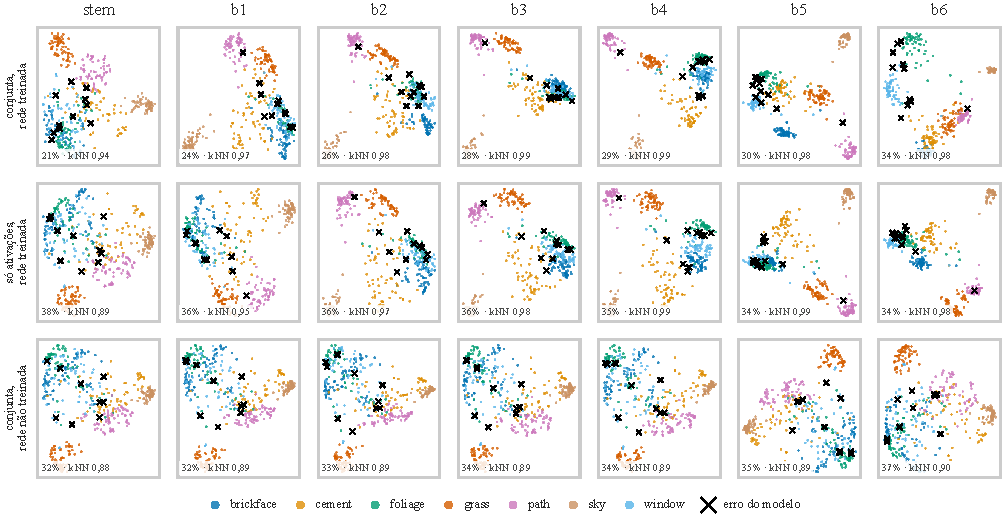
\includegraphics[width=\textwidth]{disc_espaco.pdf}
  \caption{O espaço de representação bloco a bloco, projetado nos seus dois modos dominantes, sobre as 462 amostras de teste da \texttt{segment} (perceptron multicamadas, semente 0, alvo fixo). A primeira linha mostra a Gram conjunta da rede treinada, a segunda apenas a fonte de ativações, com a mesma transformação das componentes, e a terceira a Gram conjunta da rede não treinada, com os mesmos pesos iniciais. A cor é a classe predita pela rede treinada, e os $\times$ marcam as amostras que ela erra. No canto de cada painel estão a fração da energia retida pelos dois eixos e o acerto do $k$-vizinhos contra a predição, calculado sobre a matriz de Gram inteira, e não sobre o plano.}
  \label{fig:disc_espaco}
\end{figure}

Três aspectos da figura ajudam a entender os resultados. O primeiro é o contraste entre a rede treinada e a não treinada. Na rede não treinada (terceira linha), a geometria é praticamente a mesma nos cinco primeiros blocos: a rede aleatória apenas propaga a estrutura da entrada, e as classes que já são separáveis nos atributos brutos, como \texttt{grass} e \texttt{sky}, aparecem isoladas desde o \texttt{stem}. É exatamente essa separabilidade herdada da entrada que torna o piso cruzado alto nas bases tabulares, com $k$-vizinhos em torno de $0{,}89$ nesta base. Na rede treinada (primeira linha), ao contrário, a geometria muda a cada bloco: \texttt{path}, \texttt{grass} e \texttt{sky} se destacam em grupos compactos, e as classes que a rede tem mais dificuldade de separar, \texttt{brickface}, \texttt{foliage}, \texttt{window} e \texttt{cement}, passam a ocupar uma região comum. O que distingue a medida do seu piso é, portanto, a reorganização produzida pelo treinamento, e não a separabilidade dos dados.

O segundo aspecto é a posição dos erros. Os objetos que o modelo erra não estão espalhados pelo espaço: eles se concentram na região em que as classes confundíveis se encontram, e isso ocorre em todos os blocos da rede treinada. Essa é a razão pela qual a margem geométrica prevê o acerto (P1). Um objeto cuja vizinhança mistura predições diferentes está, geometricamente, em uma fronteira, e é nas fronteiras que o modelo erra. Veja que a margem agrupa os objetos pelas predições e não recebe o rótulo do objeto, de modo que essa concentração é uma propriedade do espaço construído, e não da forma como a leitura foi desenhada.

O terceiro aspecto é a comparação entre a composição e a fonte de ativações isolada (segunda linha). Nesta base tabular, as duas geometrias são parecidas, e a composição só se distingue nos blocos rasos, o padrão que P2 encontrou nas bases tabulares. Por fim, é preciso ler a figura com uma cautela: os dois eixos retêm apenas de 21\% a 38\% da energia, de modo que objetos sobrepostos no plano podem estar separados nas demais dimensões, e é por esse motivo que o acerto do $k$-vizinhos é calculado sobre a matriz inteira.

\subsection{O que o método é capaz de fazer, e por quê}\label{subsec:res_instanciacao}

\textbf{Refletir a decisão, o erro e a semântica que o modelo expressa.} A primeira capacidade observada é a de construir um espaço em que a vizinhança de um objeto reflete como o modelo o trata e em que classes semanticamente próximas ficam próximas, mesmo sem que a hierarquia entre no treinamento (P1 e P9). Os resultados, entretanto, delimitam o alcance dessa capacidade de três formas. Nos blocos profundos, ela não é própria da composição, visto que as ativações e os próprios \textit{logits} obtêm os mesmos valores. Como sinal de confiança, a margem geométrica não supera o \textit{softmax} nem o \textit{trust score}, de modo que o espaço não antecipa o erro melhor do que o modelo já informa na sua saída. E a hierarquia semântica que as distâncias carregam é a que a confusão do próprio modelo já expressa, e não mais do que ela. As três delimitações têm a mesma origem: o método lê um espaço construído a partir do próprio modelo, e por isso reflete o seu comportamento, mas não tem acesso a uma informação que o modelo não tenha. O seu valor está, portanto, em descrever \textit{onde} e \textit{como} esse comportamento se organiza nos estados internos, e não em antecipá-lo.

\textbf{Acrescentar o gradiente às ativações onde elas ainda não decidem.} A composição supera a fonte de ativações nos blocos rasos e intermediários das redes convolucionais e se iguala a ela na saída da rede. A explicação é que as ativações descrevem o que a rede \textit{vê}, enquanto o gradiente contrastivo descreve o que \textit{importaria} para a decisão. Nos blocos profundos, as ativações das amostras de uma mesma classe tendem a colapsar em torno de uma média de classe \citep{Papyan2020} e passam a carregar a decisão por si mesmas, de modo que a composição deixa de ter o que acrescentar. No perceptron multicamadas, cuja entrada já é quase separável, e no transformador, cujo gradiente quase não carrega informação sobre a decisão, a vantagem é pequena ou inexistente. As ablações precisam essa explicação em dois pontos. Primeiro, o que acrescenta é a fonte, e não a forma multiplicativa: a composição aditiva das mesmas fontes produz as mesmas leituras que o produto de Hadamard em todas as bases, e, na ResNet do Pet, o gradiente sozinho iguala a composição. O critério de similaridade conjunta do Comentário \ref{rem:joint_similarity}, segundo o qual dois objetos só são próximos se forem próximos em todas as fontes, é, assim, uma propriedade da construção que os dados não distinguem de uma média das similaridades. Segundo, a normalização angular $T_a$ é a escolha decisiva: sem ela, a fonte de maior amplitude domina a composição e todas as leituras caem. Veja que isso delimita a instanciação, e não o método: a contribuição de cada fonte é uma propriedade do modelo analisado, e outra escolha de fontes pode ser mais informativa em outra arquitetura.

\textbf{Ver o que a CKA não vê.} A decomposição contra a CKA mostrou que a parte da Gram vista pela CKA coincide com a geometria euclidiana das ativações, de modo que a parte residual é exatamente o que uma análise das ativações não enxerga. Essa parte residual prevê o acerto melhor do que a vista nos blocos rasos e intermediários das redes convolucionais e pior nas bases tabulares e no transformador. Veja que esse é o mesmo padrão da capacidade anterior, e pela mesma razão: o que o método vê além da CKA é, essencialmente, a contribuição do gradiente. Sendo assim, o método se distingue da CKA exatamente onde a sensibilidade da decisão diverge do conteúdo das ativações.

\textbf{Concentrar a decisão em poucas direções.} A leitura espectral mais robusta é a contenção das direções de classe no subespaço retido, que supera o piso em todas as bases e arquiteturas. Isso significa que as poucas direções dominantes do espaço construído são as direções em que o modelo separa as suas decisões. A razão de energia ortogonal, que mede quanto de cada objeto vive fora dessas direções, só é confiável quando o subespaço retido já é o subespaço da decisão, isto é, nos blocos profundos das redes convolucionais e em quase todos os blocos do transformador. Em outras palavras, a energia que escapa de $V_r$ sinaliza uma amostra que o modelo não sabe representar apenas quando $V_r$ é o espaço em que o modelo decide, a mesma condição que torna útil o resíduo do subespaço principal na detecção de amostras fora da distribuição \citep{Wang2022ViM}.

\textbf{Localizar sem necessariamente explicar.} Sobre a entrada, o campo de energia da ResNet localiza o animal melhor do que um mapa centrado e do que o Grad-CAM, mas, no teste de deleção, produz uma queda de margem menor do que a do Grad-CAM a partir de \texttt{b4}. A diferença entre as duas tarefas explica o resultado. A energia de uma posição mede o quanto ela participa dos modos dominantes da geometria da imagem, isto é, da estrutura que o modelo representa, enquanto o Grad-CAM pondera cada posição diretamente pela sensibilidade da decisão. Um mapa de estrutura cobre o objeto inteiro, enquanto um mapa de sensibilidade ordena as suas partes pela importância. A localização, ademais, vem sobretudo do gradiente, o que é coerente com as capacidades anteriores. No transformador, nem a localização se sustenta, porque a atenção mistura informação de toda a imagem desde as primeiras camadas \citep{Raghu2021}, e a posição deixa de ser uma unidade natural de objeto. Na prática, o campo de energia é útil para auditar \textit{onde} uma rede convolucional representa o objeto, por exemplo para detectar um modelo que se apoia no fundo \citep{Geirhos2020}, mas não substitui um mapa de relevância quando a pergunta é quais partes sustentam a decisão.

\textbf{Explicar por contrafactuais, inclusive fora das redes neurais.} A leitura de pares responde à pergunta contrastiva, ``por que esta amostra e não aquela?'', que é a forma natural das explicações humanas \citep{Miller2019}, e o faz tomando como referência um contrafactual no sentido de \cite{Guidotti2022}: a amostra observada mais próxima que o modelo decide de outra forma. A distância do método entra em dois pontos. Ela ordena as diferenças entre a amostra e o seu contrafactual pelo quanto cada uma aproxima as duas no espaço do modelo, e cada pontuação $\Delta_f$ é o efeito de uma intervenção $do(x_f := x_{j,f})$ sobre essa distância. Nas duas bases dos estudos de caso, isso basta para superar o SHAP e o LIME, que, nas formas usuais, explicam uma amostra em relação a uma referência genérica, e não em relação ao contrafactual, e para identificar atributos informativos bem acima do acaso na verdade de base sintética. Não basta, contudo, para alcançar as decomposições exatas da variação da margem entre as duas amostras, o valor de Shapley com $j$ de referência e os gradientes integrados, que vencem o método em todos os testes. A razão é que essas técnicas decompõem diretamente a quantidade que o teste mede, enquanto o método a aproxima por uma distância em uma representação interna. A verdade de base sintética, que não favorece nenhuma técnica por construção, confirma essa leitura: nela, a diferença entre os gradientes integrados e o método cai para cinco pontos percentuais ($0{,}65$ contra $0{,}60$), de modo que boa parte da vantagem das decomposições no teste de trocas vem de medirem a própria quantidade testada. Visto de outro modo, o método se aproxima da atribuição com fundamento axiomático, o valor de Shapley com $j$ de referência, que é a única a satisfazer eficiência, simetria, nulidade e linearidade para o jogo da troca \citep{SundararajanNajmi2020}: os dois rankings têm correlação de Spearman mediana de $0{,}81$ e $0{,}84$ e o mesmo atributo principal em 75\% e 80\% dos pares, e o método chega a isso sem consultar a saída do modelo, apenas pela geometria de um bloco intermediário. Em relação ao valor exato, essa aproximação tem uma vantagem de custo que cresce exponencialmente com o número de atributos: o método avalia $F + 2$ linhas por par, contra $2^F$ do Shapley exato, isto é, 18 contra $65\,536$ avaliações com os dezesseis atributos destas bases, e o seu custo medido permanece linear até milhares de atributos, enquanto o exato dobra a cada atributo acrescentado e se torna inviável a partir de algumas dezenas (Subseção \ref{subsec:res_custo}). Essa vantagem, contudo, não se estende às estimativas baratas da mesma quantidade: o Shapley estimado por poucas permutações tem custo linear, como o método, e os gradientes integrados têm custo constante em $F$, e as duas ficam acima do método no teste de trocas. Os gradientes integrados, por sua vez, exigem que o modelo seja diferenciável em relação à entrada e não se aplicam, por exemplo, à árvore de decisão, à qual o método se aplica apenas com outra escolha de fontes. O que distingue o método dessas estimativas é o que a distância permite e as decomposições da saída não oferecem: a datação por bloco do atributo que separa as duas amostras.

O resultado mais forte vem da árvore de decisão, em que a resposta certa é conhecida e o método a recupera sem receber a regra de decisão, apenas trocando as fontes. A recuperação sobrevive à remoção da fonte de caminho, que já codifica o nó de separação, e a datação não se altera sem ela, nas duas bases. Esse é o argumento mais direto de que o método é modelo-agnóstico, no sentido de que a construção se aplica a modelos de natureza distinta: ela exige somente que cada amostra possa ser descrita por fontes sobre as quais se define um \textit{kernel}, e o que depende do modelo é apenas a instanciação.

\textbf{Datar a decisão.} As leituras por bloco produzem uma datação da decisão, e nas redes essa datação concorda com a obtida por intervenção sobre os estados internos. Parte dessa concordância decorre de as duas séries crescerem com a profundidade, mas, nas bases tabulares e no Pet, ela sobrevive à remoção da tendência: os blocos em que a decisão mais se estabiliza são aqueles em que a geometria mais ganha. No CIFAR-100, a concordância sem tendência não se distingue de zero, de modo que a datação por bloco não é, sozinha, uma validação. A verificação mais direta veio da árvore, em que a profundidade da decisão é conhecida para cada par. Uma consequência prática é que a leitura por bloco permite localizar em que ponto do modelo uma distinção passa a ser usada, uma informação que atribuições sobre a saída do modelo não oferecem.

\subsection{Quando o método não é capaz, e por quê}\label{subsec:disc_limites}

Três limites decorrem da própria construção das leituras, e não de detalhes de implementação.

O primeiro é que a leitura de pares é de primeira ordem. A pontuação $\Delta_f$ intervém em um atributo de cada vez, e os atributos que só importam em conjunto não mudam nada quando trocados sozinhos. Por isso o método recupera o atributo que separa a amostra do seu contrafactual, mas não o contrafactual mínimo, isto é, o menor conjunto de mudanças que altera a decisão, e o valor de Shapley com $j$ de referência, que considera todas as combinações de trocas, o supera no teste de trocas. Em outras palavras, o método explica o que distingue duas instâncias, e não como transformar uma na outra com o menor custo, que é o objetivo dos geradores de contrafactuais \citep{Wachter2018, Guidotti2022}. Uma extensão natural do método é substituir a troca isolada por trocas sequenciais, recalculando a distância depois de cada uma, o que capturaria interações e manteria o custo linear no número de atributos.

O segundo é que o método depende de o treinamento reorganizar a geometria. Se a tarefa é resolvida quase na entrada, a rede treinada e a não treinada produzem espaços parecidos, e as leituras se aproximam do que a diferença bruta entre as amostras já dizia. É o que se observa nas bases tabulares, em que o piso cruzado é alto e a leitura de pares empata com a diferença bruta $|\Delta x|$, e é coerente com a Figura \ref{fig:disc_espaco}, em que a vantagem sobre o piso é justamente a reorganização entre os blocos. A similaridade entre a Gram da rede treinada e a da rede na inicialização é barata e poderia ser reportada antes de qualquer leitura, como um diagnóstico de aplicabilidade, mas esse critério ainda precisa ser validado sobre um número maior de bases.

O terceiro é que a validade das leituras referidas à decisão depende da escolha do alvo do gradiente. Com a classe predita como alvo, o gradiente carrega a própria predição, e as leituras de decisão se tornam circulares, chegando a recuperar a predição em mais de 95\% dos casos já em \texttt{b3} da ResNet do Pet. O alvo fixo remove essa circularidade ao custo de tornar o gradiente degenerado no último bloco. Essa é uma restrição da fonte de gradiente, e não do método, mas qualquer instanciação que utilize a decisão como fonte precisa de um controle equivalente.

\subsection{Limitações e trabalhos futuros}\label{subsec:res_limitacoes}

\noindent\textbf{Sobre o termo ``mecanicista''.} A interpretabilidade mecanicista é o estudo dos mecanismos computacionais internos de um modelo, seus componentes, sua organização funcional e estrutural \citep{Kastner2024}. O Fannar contribui para esse conjunto de métodos por explorar padrões de semelhança nas representações internas do modelo (através dos \textit{kernels}) e utilizar a geometria definida por essas semelhanças para interpretar seu comportamento. Por ser centrado no reconhecimento de padrões da organização interna do modelo e por não identificar, por si só, os componentes funcionais relevantes nem reconstruir como suas interações implementam o comportamento do modelo, ele constitui um método mecanicista de escopo delimitado.

A proposição de que as distâncias do espaço de representação refletem o entendimento que o modelo tem dos dados foi avaliada em duas dimensões: a comportamental (P1 a P8) e, em P9, a semântica, contra a hierarquia de classes das duas bases de imagens. Na segunda, a hierarquia das distâncias não excede a que a confusão do modelo já expressa, de modo que a afirmação de que as distâncias representam diferenças semânticas além do comportamento permanece sem sustentação. Referências semânticas mais ricas, como julgamentos humanos de similaridade, não foram utilizadas.

Do ponto de vista experimental, as limitações se dividem em três grupos. O primeiro é a escala das imagens. Todos os modelos são treinados do zero. No Pet, o regime de dados escassos, com cerca de noventa imagens por raça, limita a acurácia, sobretudo a do transformador ($0{,}44$). Treinar a partir de pesos pré-treinados elevaria essa acurácia, e o piso passaria a ser a mesma rede com os pesos reinicializados \citep{Adebayo2018}. Essa extensão é necessária para sustentar as conclusões sobre transformadores. Além disso, com oito sementes por arquitetura, uma comparação nas imagens só é significativa quando se sustenta em quase todas as sementes, e nenhuma sobrevive à correção sobre os sete blocos de uma afirmação, de modo que as comparações nas imagens permanecem descritivas.

O segundo grupo é o alcance dos estudos de caso. Eles utilizam duas bases tabulares com dezesseis atributos, escolhidas para que o valor de Shapley exato fosse calculável, e uma verdade de base sintética com uma única estrutura (atributos informativos independentes e ruído). Bases com mais atributos, interações conhecidas entre eles e outras famílias de modelos ampliariam essa comparação.

O terceiro grupo são escolhas da instanciação que não foram variadas: a regra $r=Q-1$ não teve a sua sensibilidade avaliada, o piso adotado na diagonal da transformação angular não foi variado, os conjuntos de nível foram validados apenas na ResNet do Pet e a seleção da posição de referência ainda não exclui a borda da imagem. Por fim, a conexão entre a decomposição empírica e o operador de Mercer é assintótica (Subseção \ref{subsec:spectral}).

Além das extensões já mencionadas, a leitura de pares por trocas sequenciais e a decomposição espectral truncada para amostras maiores, três direções decorrem diretamente dos resultados. A primeira é explorar outras fontes para as arquiteturas em que o gradiente pouco contribui, como o transformador, em que a atenção é uma candidata natural a fonte. A segunda é tomar a equivalência entre o produto de Hadamard e a soma como ponto de partida: ela indica que, nas fontes utilizadas, a informação está nas fontes e na sua normalização, e não na forma de compô-las, e uma instanciação com fontes menos correlacionadas entre si é o caso em que a similaridade conjunta poderia fazer diferença. A terceira é utilizar o método para comparar modelos diferentes sobre as mesmas amostras, como a árvore de decisão e o perceptron multicamadas da \texttt{letter}, colocando os dois na mesma geometria e perguntando não apenas se eles usam os mesmos atributos, mas se organizam os dados da mesma forma.
